\chapter{Model and General Principles}
\label{ch:background}

This chapter will discuss the model and general principles, which serve the foundation to understand the implementation reports of the following chapter. Its important to understand every subsection of this chapter, such as the ethereum blockchain, \ac{PoW}, the \ac{EVM} and all topics needed for atmoic cross-chain swaps. 

% MB NOT HERE - - write about bitcoin and what changes it brought - buterin eth paper

%
% Section: Der erste Abschnitt
%
\section{Ethereum Blockchain}
\label{sec:background:first_section}
The Ethereum blockchain was introduced in Vitalik Buterin’s paper in 2013, which addressed several limitations of the Bitcoin’s scripting language \cite{buterin2013ethereum} based on Buterin's white paper Wood released the yellow paper one year later \cite{wood2014ethereum}. The main contributions are full Turing-completeness and saving all states of computations in between the states \cite{dannen2017introducing}.
Through its own programming language Solidity, it provides an abstract layer enabling anyone to create their own rules for ownership, formats of transactions, and state transition functions \cite{vujivcic2018blockchain}. Development was funded by an online crowdsale that took place between July and August 2014 \cite{tapscott2016blockchain}. The system then went live on 30 July 2015 \footfullcite{"Ethereum Launches" - https://blog.ethereum.org/2015/07/30/ethereum-launches/. Retrieved 30 July 2015} and is called the ethereum public blockchain. Which means its accessible to everyone who wants to send Ether token or execute smart contracts. In general we have to distinguish between private and public blockchains. The public one is described above. Since everybody can go to github and fork e.g the geth client its possible to start an own private blockchain. In an enterprise software context, where corporate stakeholders are given certain rights and privileges to read and write to the company chain, the deployment is known as a permissioned blockchain. Nevertheless for both the private (permissioned) and the public blockchain its possible to do the following \cite{dannen2017introducing}:

\begin{itemize}
	\item Send and receive Ether
	\item Write smart contracts
	\item Create provably fair applications
	\item Launch your own token based on Ether
\end{itemize}

% ADD LINEBREAK TO FOOTNOTE AND ADD THIS AT THE BEGINNING   Foundation, Ethereum 

\clearpage

\subsection{Proof-of-Work Consensus Algorithm}
\label{subsec:background:first_section:second_subsection}

%MB check wood paper for more historical PoW data!!

The \ac{PoW} system of bitcoin and ethereum is similar to Adam Back's Hashcash \cite{back2002hashcash}, but instead of a newspaper or Usenet post the \ac{PoW} involves scanning for a value, which is hashed with the \ac{SHA-256} to begin with a number of zero bits. The average work required is exponential. Which means the more leading zeros, the more work. In the end the work can be later verified by executing a single hash. The \ac{PoW} is implemented by incrementing a nonce in the block until a value is found that gives the block's hash the required zero bits. The majority decision is represented by the longest chain, which has the greatest \ac{PoW} effort invested in it. Because later blocks are chained after the premature block, the work to change the block would include redoing all the blocks after it. To modify a past block, an attacker would need to redo all the past work until the specific block he wants to change \cite{nakamoto2008peer}. 

\begin{figure}[h]
	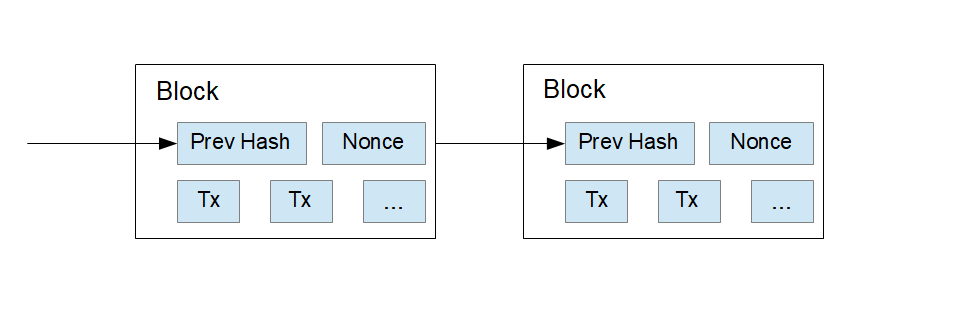
\includegraphics[height=4cm]{blocks}
	\caption{Blocks}
	\label{fig:blocks}
\end{figure}

Beginning with the genesis block, each single block is chained to the previous block by including the the previous hashes (figure \ref{fig:blocks}). The \ac{SHA-256} takes a 256 bit length of input
messages and hash them to fixed-length outputs \cite{van2014encyclopedia}. So the \ac{SHA-256} function starts by padding the message according to the so-called Merkle-Damg{\aa}rd strengthening technique. Further the message is processed block by block with the the underlying compression function, which initializes an appropriate number of chaining variables to a fixed value to hash the genesis block and also the current hash value for the following blocks \cite{coron2005merkle}. In the year 2003 the \ac{SHA} was published by the \ac{ISO} making \ac{SHA} a standard for most countries in the world \cite{isoSHA-256}. Five years later Satoshi Nakamoto proposed the first concept of a \ac{PoW} based blockchain to allow for public agreement on the order of transactions. The public ethereum blockchain uses \ac{PoW} to this day. There are several other consensus algorithms today suitable for a blockchain and some are considered to be an improvement to \ac{PoW}, which will be discussed later in this work.

\clearpage

\subsection{Ethereum Virtual Machine}
\label{subsec:background:first_section:ethereum}
This chapter will cover basics of the \ac{EVM} and discuss the transaction execution to reach a general understanding what the \ac{EVM} is and how it works. The \ac{EVM} is a simple stack-based architecture. The word size of the machine is 256-bit and the stack has a maximum size of 1024 elements, meaning that the \ac{EVM} can store a total of 1024 stack items with each 256-bit. The machine does not follow the standard von Neumann architecture. Rather than storing program code in generally-accessible memory or storage, it is stored separately in a virtual ROM. The \ac{EVM} is different from the von Neumann architecure, because it can have exceptional execution thus as the out-of-gas exception. \cite{wood2014ethereum} The ethereum network can be seen as one single computational device, where the point of turning the machine on is the creation of the genesis block. All blocks of a blockchain hold information about state changes of the \ac{EVM}, the ethereum public blockchain holds all state transitions of the \ac{EVM} since it was initially turned on. Since every state transition of the \ac{EVM} is modelled as a transaction, a blockchain holds the whole history of states of the specific machine \cite{dannen2017introducing}. Before it will be put into a block each transaction is verified and validated before the next canonical block can be placed on the last one. Through the transaction validation, nodes on the network do not need to individually evaluate the trustworthiness of every single block in the network to compute the present balances of the accounts on the network. The client simply has to verify the hash of the parent block and see if the new block contains the correct hash its parent’s transactions and state \cite{dannen2017introducing}. The current valid block in an ethereum network is known as world state (state), which is a mapping between addresses (160-bit identifiers) and account states. Thus being the current executional state of the virtual state machin, knwon as the \ac{EVM}. It is considered as a quasi-Touringcomplete virtual machine. Since the amount of total execution is intrinsically bound to the parameter gas, the quasi  qualification is added \cite{wood2014ethereum}. The execution model is defined by the ethereum state transition function and specifies how system state is altered through bytecode executions. \newline \newline
The ethereum state transition function, APPLY(S, TX) -> S' is defined by Buterin \cite{buterin2013ethereum}  as follows:

\begin{enumerate}
	\item Check for transaction and signature validity and check if the nonce of the sender account matches the receivers account's nonce. If not, return an error.
	\item Calculate the transaction fee and determine the sending address from the signature. Increment the sender's nonce and substract the fee from the sender's account. Return an error, if the balance of the sender's account is lower than the fee.
	\item Initialize GAS including a certain quantity of gas per byte to pay for the bytes in the transaction.
	\item If the receiver's account doesnt exist, create it and then send the transaction value from sender's account to the receiver. If the receiver's account is a contract, run code execution until completed or gas is depleted.
	\item In case the value transfer or code execution failed because theres not enough gas, revert all state changes except the payment of the fees and add the fees to the miner's account.
	\item If code execution has completed refund the fees for all remaining gas to the sender and also send the fees paid for gas consumed to the miner.
\end{enumerate}


\begin{figure}[h]
	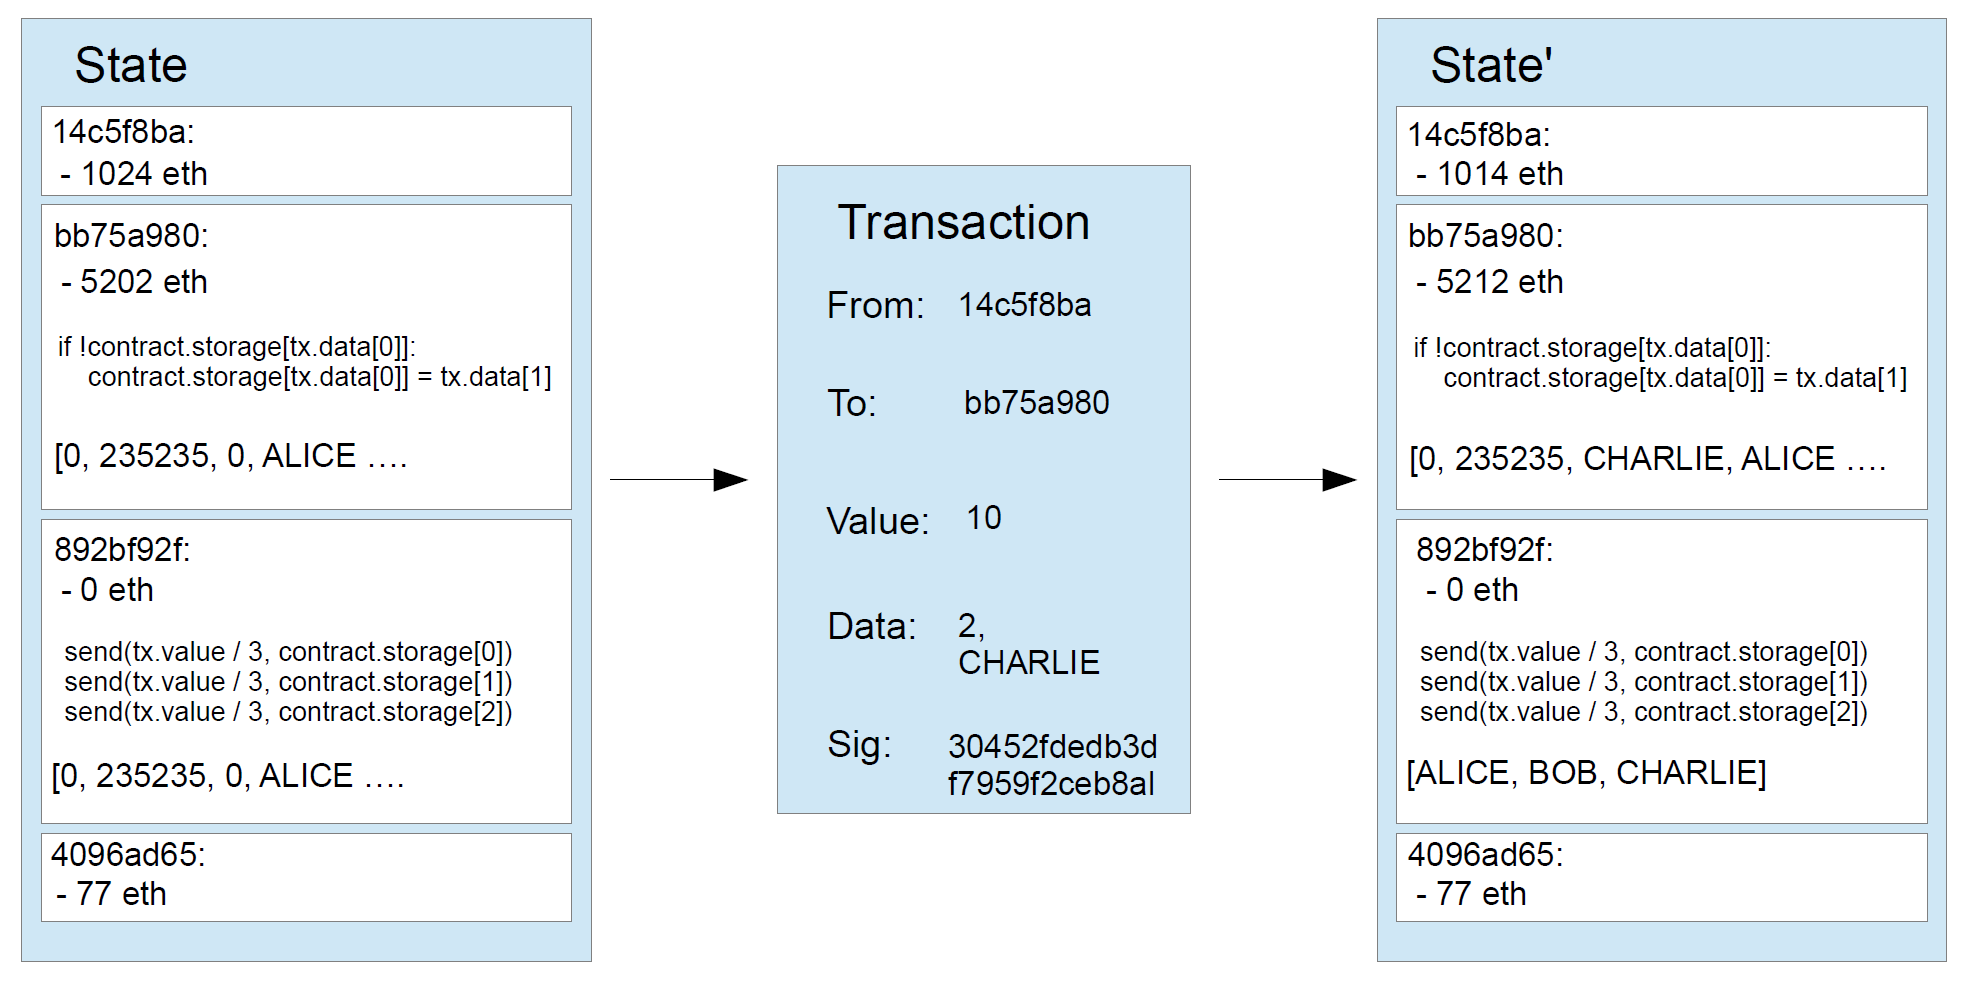
\includegraphics[width=14cm]{ethereum_state_transition_function}	%16cm
	\caption{Ethereum State Transition Function}
	\label{fig:ethereum_state_transition_function}
\end{figure}
% BRING REAL EXAMPLE WITH CALCULATIONS OF GAS?

The Figure above shows all calculations applying the function APPLY(S, TX) -> S' to an example state (figure \ref{fig:ethereum_state_transition_function}). Due to the distributed nature of the \ac{EVM} and the fact its built of many nodes around the world. Meaning to ensure distributed security, it must be purpose-built to solve the diffmatching problem that can occur, when there are many near-simultaneous changes to the same database from many actors in the system all around the world \footfullcite{Google Code "Diff-Match Patch" - https://code.google.com/p/google-diff-match-patch/ 2016}. Solving this problem in a verifiable and trustworthy way is basically what the \ac{EVM} does. It's resilience and security does increase with the amount of machines in the network and is implemented and backed by the gas fee system. The opportunity to earn gas as a miner is one reason for many nodes to participate in the network and at the same time raises security \cite{dannen2017introducing}.

% MB add that there are opcodes and stuff, like any other machine has, but not covered here(would go too deep)
%- explain how code execution works on a distributed system

%ueberleitung von execution model erledigt zur smart contract 
 
\clearpage


\subsection{Smart Contracts}
\label{subsec:background:first_section:first_subsection}

Mark Miller. The Future of Law. In paper
delivered at the Extro 3 Conference (August 9),
1997. URL https://drive.google.com/file/d/0Bw0V
XJKBgYPMS0J2VGIyWWlocms/edit?usp=sharing.

Nick Szabo. Formalizing and securing relationships on
public networks. First Monday, 2(9), 1997. URL
http://firstmonday.org/ojs/index.php/fm/art
icle/view/548. https://web.archive.org/web/
20170810042659/http://firstmonday.org/ojs/inde
x.php/fm/article/view/548.

Early work on smart contracts has been done by Szabo
[1997] and Miller [1997]. Around the 1990s it became clear
that algorithmic enforcement of agreements could become
a signicant force in human cooperation. Though no speci
c system was proposed to implement such a system,
it was proposed that the future of law would be heavily
%5aected by such systems. In this light, Ethereum may
be seen as a general implementation of such a crypto-law
system.
in ethereum context by wood known simple known as contracts \cite{wood2014ethereum}

buterin first introduced the term smart contracts \cite{buterin2013ethereum}

The Name “Smart Contracts”
Rather than bore you with the etymology of this word, let’s clear up one thing: in this
context, contract refers to a specific kind of contract: a financial contract, also known
more colloquially as a derivative, or option. Financial contracts are agreements to buy
and sell at some point in the future, usually at a specified price. In the Ethereum context,
smart contracts are agreements between accounts, to render a transfer of ether (that is, a
payment) when certain conditions are met.
The reason these contracts are “smart” is that they’re executed by machine, and
the assets (ether or other tokens) are moved automatically. These contracts could be
enforced even hundreds of years after they’ve been written, assuming the network is
still running then—and even if a lot of bad actors try to interfere. The EVM is totally
sandboxed and free from interference, and isolated from other networks too, making it
impossible for a party to back out of a smart contract. In practical terms, this is because
smart contracts are empowered to hold assets (ether or other tokens) in escrow and move
them when the terms of the contract are met.
The EVM Runs Bytecode
The EVM has its own language, the EVM bytecode, to which your smart contracts compile.
Solidity, which is a high-level language, is compiled into bytecode and uploaded onto the
Ethereum blockchain by using a client application such as the Mist browser or a full node.\cite{dannen2017introducing}



- important! solidity is a high level programming language, code execution on the evm directly is known as bytecode


\clearpage


\section{Digraphs}
\label{sec:background:second_section}
EXPLAIN DIGRAPHS HERE
\cite{bang2007theory}

\section{Hashlocks and Timelocks}
\label{sec:background:third_section}
EXPLAIN HASH AND TIMELOCKS HERE


\section{Atomic Cross-Chain Swaps}
\label{sec:background:fifth_section}

theres also research specifically for ethereum private sidechains \cite{robinson2019atomic}
EXPLAIN ATOMIC CROSS CHAIN SWAPS HERE
\cite{herlihy2018atomic}